\documentclass[a4paper]{article}
\usepackage[margin=8mm]{geometry}

\usepackage{tikz,pgfplots}
\usetikzlibrary{matrix}
\pgfplotsset{compat=1.12}
\usepgfplotslibrary{external} % creates a tight self-contained pdf figure for each tikzpicture
\tikzexternalize % comment out to debug if latex errors: generates the external pdf
\tikzset{external/force remake} % otherwise will use external pdf if it exists
\tikzset{png export/.style={
	external/system call={
		% print some info to console
			echo "\\n---- Checking Imagemagick/convert available ----\\n\\nPATH:" $PATH "\\n";
			which convert; echo; convert -version;
		pdflatex \tikzexternalcheckshellescape
			-halt-on-error -interaction=batchmode -jobname "\image" "\texsource";
		% convert from pdf to png
		convert -units pixelsperinch -density 150 "\image.pdf" "\image.png";
		convert -units pixelsperinch -density 600 "\image.pdf" "\image-600.png";
}}}
\tikzset{png export}
\tikzsetexternalprefix{figures/} % output the pdf to an existing directory (needs to exist)
\tikzsetnextfilename{myfigure}

\begin{document}

\section*{tikzpicture to be externalized to pdf and converted to png(s)}

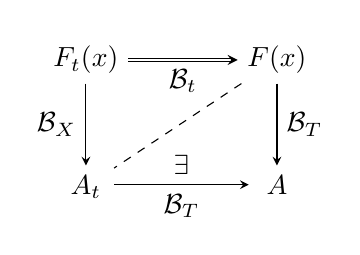
\begin{tikzpicture}
	\matrix (m) [matrix of math nodes,row sep=3em,column sep=4em,minimum width=2em]
	{ F_t(x) \pgfmatrixnextcell F(x) \\
		A_t \pgfmatrixnextcell A \\};
	\path[-stealth]
		(m-1-1) edge node [left] {$\mathcal{B}_X$} (m-2-1)
						edge [double] node [below] {$\mathcal{B}_t$} (m-1-2)
		(m-2-1.east|-m-2-2) edge node [below] {$\mathcal{B}_T$}
						node [above] {$\exists$} (m-2-2)
		(m-1-2) edge node [right] {$\mathcal{B}_T$} (m-2-2)
						edge [dashed,-] (m-2-1);
\end{tikzpicture}

\section*{Checking quality and size of converted png(s)}

Check that the native figure size is correct by importing the generated png(s) \emph{without scaling}.

\subsection*{150dpi figure}
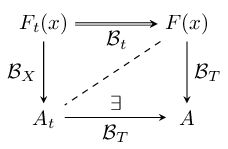
\includegraphics{figures/myfigure.png}

\subsection*{600dpi figure}
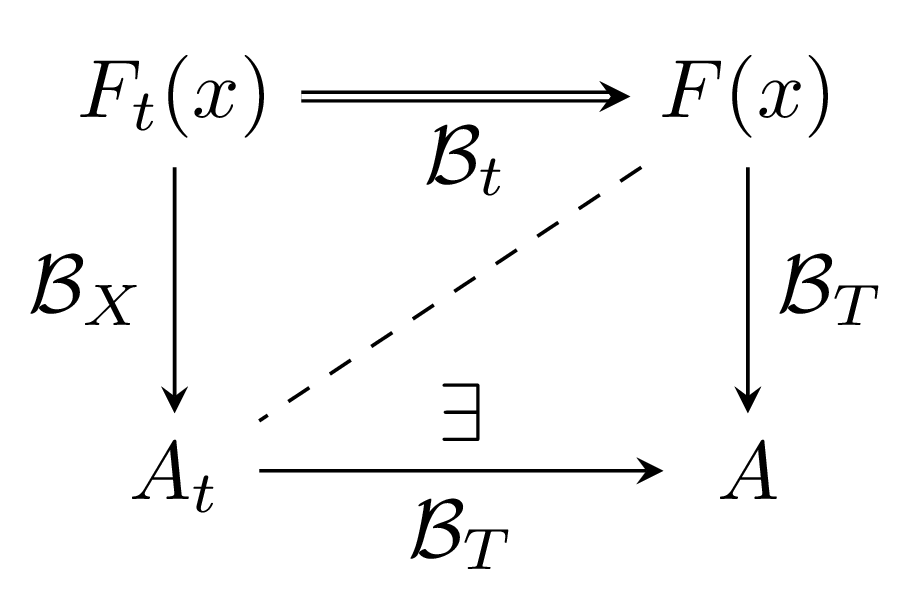
\includegraphics{figures/myfigure-600.png}

\end{document}